\documentclass[journal,12pt,twocolumn]{IEEEtran}
\usepackage{graphicx}
\graphicspath{{./images/}}
\usepackage{amsmath,amssymb,amsfonts,amsthm}
\newcommand{\myvec}[1]{\ensuremath{\begin{pmatrix}#1\end{pmatrix}}}
\usepackage{listings}
\usepackage{watermark}
\usepackage{titlesec}
\let\vec\mathbf
\lstset{
frame=single, 
breaklines=true,
columns=fullflexible
}
\thiswatermark{\centering \put(0,-105.0){
\includegraphics[scale=0.2]{/sdcard/IITH/matrix/circle/figs/logo.png}} }
\title{\mytitle}
\title
{
Matrix Assignment - Circle
}
\author{Surajit Sarkar}
\begin{document}
\maketitle
\tableofcontents
\bigskip


\section{\textbf{Problem}}
Consider a family of circles passing through two fixed points A(3,7) and B(6,5) show that the chords in which the circle $x^2+y^2-4x-6y-3=0$ cuts the members of the family are concurrent at a point.Find the coordinates of this point ?
\section{\textbf{solution}}
\begin{align}
    \vec{x}^2+\vec{y}^2-9\vec{x}-12\vec{y}+53&=0\\
    \vec{x}^{\top}\vec{V}_1\vec{x}+2\vec{u}_1^{\top}\vec{x}+f_1&\\
    \vec{x}^{\top}\myvec{1&0\\0&1}{\vec{x}+2\myvec{\frac{-9}{2}}-6}\vec{x}+ 53&=0
\end{align}
Where
\begin{align}
    \vec{V}_1&={\myvec{1&0\\0&1}}\\
    \vec{u}_1&={\myvec{{\frac{-9}{2}}-6}}\\
    f_1&=53
\end{align}
Equation of circle with A and B as diameter\\
Equation of line passing through A and B
\\ 
\\Direction vector  
  \begin{align}
    \vec{m= A-B}
\end{align}
\\Normal vector
\begin{align}
    \vec{n} = \vec{R}_{\frac{\pi}{2}} \myvec{\Vec{m}}
\end{align}
where
\begin{align}
\vec{R}_{\frac{\pi}{2}} =\myvec{\cos\theta&-\sin\theta\\ \sin\theta&\cos\theta}
\end{align}
Equation of $L_1$
\begin{align}
    \vec{n}^T{\myvec{\vec x-\vec A}}&=0\\
    \vec {n^T x}-\vec {n^TA}&=0
\end{align}
Given circle
\begin{align}
    \vec{{x}^2+{y}^2}-4{\vec x}-6{\vec y}-3&=0\\
    \vec{x}^{\top}\vec{V}_2\vec{x}+2\vec{u}_2^T\vec{x}+f_2&\\
    \vec{x}^{\top}\myvec{1&0\\0&1}\vec{x}+2\myvec{-2&-3}\vec{x}-3&=0
\end{align}
Where
\begin{align}
    \vec{V}_2&=\myvec{1&0\\0&1}\\
    \vec{u}_2&=\myvec{-2&-3}\\
    f_2&={-3}
\end{align}
Common chord is given by
\begin{align}
    \vec{c}_1-\vec{c}_2+\lambda{L_1}
\end{align}
Where\\ $c_1$ is circle having A and B as diameter\\
        $c_2$ is given circle
\begin{align}
\myvec{-5&-6}\vec{x}+56+\lambda L_1\\
\myvec{5&6}\vec{x}=56---\myvec{L_2}
\end{align}
Using python we get the $L_1$ and intersection point
\begin{align}
    \vec{\myvec{2&3}}{\vec x}&=27 ---\myvec{L_1}\\
    \vec{\myvec{5&6\\2&3}}{\vec x}&={\myvec{56\\27}}\\
    \vec{x}&={\myvec{2,7.667}}
\end{align}
\section{\textbf{Code Link}}
\begin{lstlisting}
https://github.com/sssurajit/fwc/blob/main/matrix/circle/codes/circle.py
\end{lstlisting}
Execute the code by using the command
\\ \textbf{python3 circle.py}
\section{\textbf{Figure}}
\begin{figure}
    \centering
    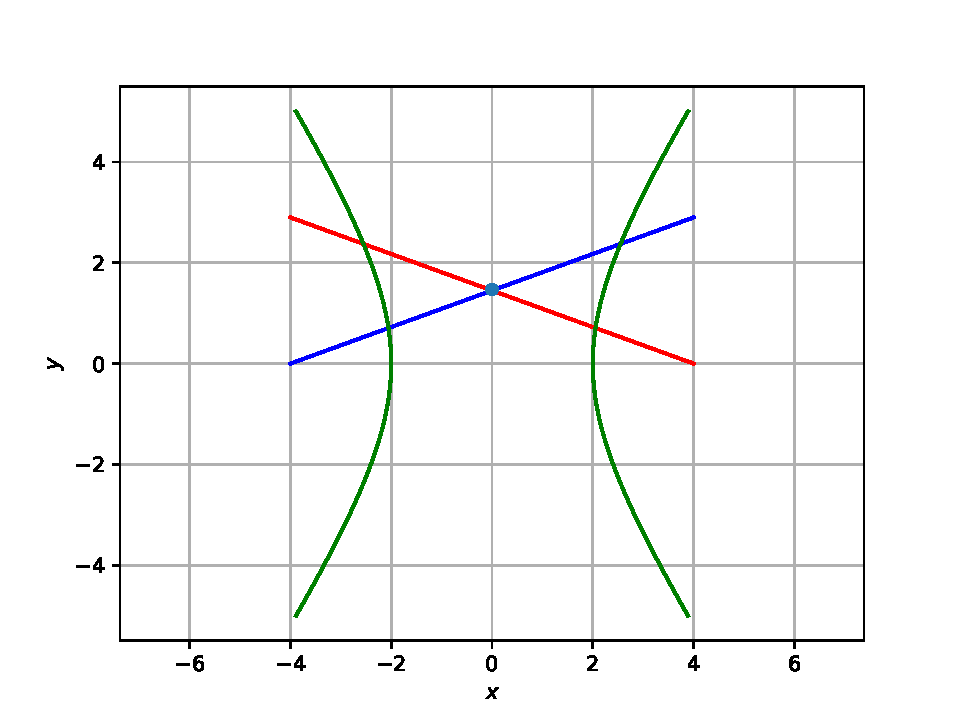
\includegraphics[width=\columnwidth]{/sdcard/IITH/matrix/circle/figs/fig.pdf}
    \caption{}
    \label{fig}
\end{figure}
\end{document}
